\chapter{Algorithms} \label{Algorithms}

In this chapter, we will show two new algorithms which combined with the two-pass algorithm described in Chapter \ref{two-pass_algorithm} \cite{chladek_thesis} can be used to obtain the most parsimonious isometric gene tree reconciliation. This approach is then implemented in our software.

The required input for our overall approach is a rooted species tree with exact branch lengths and an unrooted gene tree with inexact branch lengths. The input is processed by the following algorithms. Using our first algorithm, we select a set of possible roots of the gene tree and root the gene tree, which results in multiple rooted gene trees. Afterwards, for each rooted gene tree, we perform the two-pass algorithm to find a reconciliation  (Chapter \ref{two-pass_algorithm}) and use our second algorithm to count the number of duplications and gene losses in the found reconciliation. Finally, we select the most parsimonious reconciliation among those considered. Note however that this  reconciliation may not be optimal, as we do not try all possible roots, and our selected set of considered roots may not contain the optimal one. We allow only evolutionary events of duplication, gene loss and speciation can happen in evolutionary history.

\section{Rooting the gene tree} \label{rooting_the_gene_tree}

An unrooted gene tree has an infinite number of possible root locations. We present an algorithm to select a finite set of possible roots that are spaced by a given step on every edge $e$ of an unrooted gene tree $G$. However, our set of possible roots may not always contain the optimal solution. 

For each edge $e \in E(G)$, we transform the unrooted gene tree into a semi-rooted gene tree by rooting the subtrees at vertices $u \in V(G)$ and $v \in V(G)$ of the edge $e = (u, v)$. The edge is subsequently used as the parameter for the Algorithm~\ref{getIntervals} to select a set of roots on edge $e$, each root given by a pair of intervals. Let $r$ be the root of a semi-rooted gene tree $G$ then the first interval of the pair represents the length of edge $(u, r)$ and the second interval represents the length of edge $(r, v)$.

\begin{algorithm}[!htbp]
\caption{Possible intervals to subdivide given edge $e$} 
\label{getIntervals}
\begin{algorithmic}[1]
\Function{getIntervals}{$e \in E(G), step \in R$}
	\State intervals.add($[ \epsilon, \epsilon ]$, $[ w(e)_{min}-\epsilon, w(e)_{max}-\epsilon ]$) 
	\State intervals.add($[ w(e)_{min}-\epsilon, w(e)_{max}-\epsilon ]$, $[ \epsilon, \epsilon ]$)

	\State difference = $w(e)_{min} - w(e)_{max}$
	\If {step $>$ difference / 2}
		\State intervalSize = difference / 2
	\Else
		\State intervalSize = step
	\EndIf
	\State $w(u,r)_{min}$ = $w(e)_{min}$
	\State $w(u,r)_{max}$ = $w(e)_{max}$ - intervalSize
	\State $w(r,v)_{min}$ = $\epsilon$
	\State $w(r,v)_{max}$ = intervalSize
	
	\If {$step > 0$}
	\While {$w(r,v)_{max} < w(e)_{max}$ \textbf{and} $w(u,r)_{max} > 0$}
		\State intervals.add($[w(u,r)_{min}, w(u,r)_{max}]$, $[w(r,v)_{min},w(r,v)_{max}]$)
		\State $w(u,r)_{min}$ -= step
		\If {$w(u,r)_{min} \le 0$}
			\State $w(u,r)_{min}$ = $\epsilon$
		\EndIf
		\State $w(u,r)_{max}$ -=step
		\State $w(r,v)_{min}$ += step
		\State $w(r,v)_{max}$ += step
	\EndWhile

	\EndIf
	\Return {intervals}
\EndFunction
\end{algorithmic}
\end{algorithm}

At the beginning of Algorithm \ref{getIntervals}, we define essential variables. The set of possible pairs of intervals for subdividing the edge $e$ are stored at the variable \emph{intervals} that is also the return value of the function.

To cover most of the possibilities, we allow rooting the gene tree right above the vertices $u$ and $v$ of the edge $e$ with $\epsilon$ distance from the vertices. The $\epsilon$ is by default set to \num{1e-6} and signifies the edge length close to the $0$. We do not allow $0$ edge length or interval starting with $0$ as $[0, \epsilon]$ to avoid mapping the root into vertex $u$ or $v$.

We get two possible roots after subdividing the edge $e$ right above the vertices $u$ and $v$. The first possible root subdivides edge $e$ into two edges with interval lengths $w(u, r) = [ \epsilon, \epsilon ]$ on the left from the root and $w(r, v) = [ w(e)_{min}-\epsilon, w(e)_{max}-\epsilon ]$ on the right from the root, where $w(e)_{min}$ is original minimal length of the edge $e$ and $w(e)_{max}$ is original maximal length of the edge $e$. The second option of the root subdivides the edge $e$ with intervals of the lengths that are flipped, so the original interval $w(u, r) = [ w(e)_{min}-\epsilon, w(e)_{max}-\epsilon ]$ is on the left from the root and $w(r, v) = [ \epsilon, \epsilon ]$ in on the right from the root.

After creating the first two options for the possible root, we prepare variables for the while loop. We added a condition for special cases, where the difference between the maximal and minimal original length of edge $e$ divided by $2$ is less than the size of the step. With the special case condition, we can create intervals that would be otherwise skipped (Fig. \ref{finding_root}). We run a while loop to get possible roots inside the edge $e$. In each iteration, we subtract the step from the minimal and maximal length of the left interval of the subdivided edge $e$ and add the step to the minimal and maximal length of the right interval of the subdivided edge $e$. The size of the step is set to $0.01$ by default. The while loop goes until the maximal length of the right interval is the same or bigger as the original maximal length of the edge $e$ or the maximal length of the left interval reaches $0$ or less.

\begin{figure}[!htbp]
	\centering
  	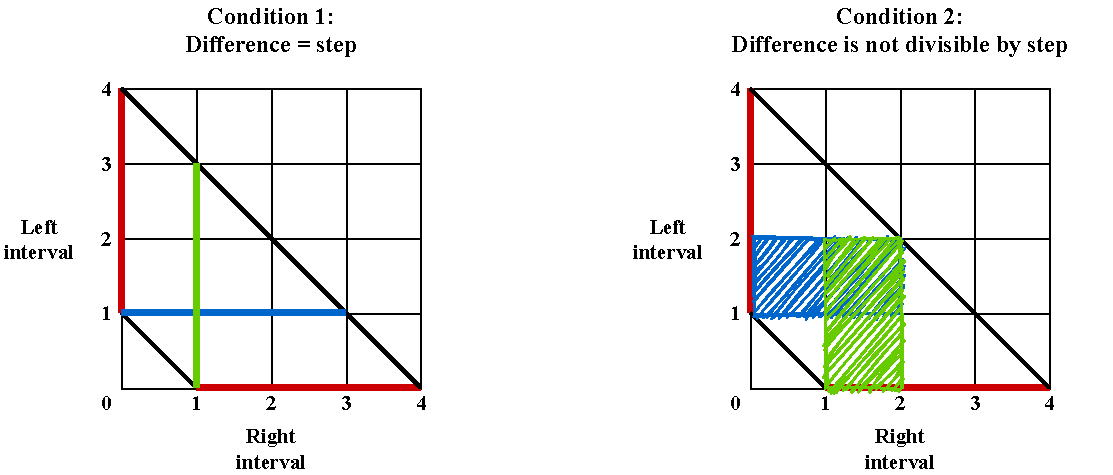
\includegraphics[width=\linewidth]{finding_root}
  	\caption[Rooting the gene tree]
  	{The X-axis on the graph stands for the possible length of interval on the right from the root and the y-axis signifies the possible length of interval on the left from the root. The space between the black diagonal lines represents all possible intervals after subdividing the edge $e$ with the root. The red lines represent the first two pairs of intervals added to the solution, corresponding to the root right above the vertices $u$ and $v$, where one interval takes the original size and the second interval is $[\epsilon, \epsilon]$. Blue rectangles represent  pairs of intervals for the root inside the edge $e$ without the special case condition. Green squares are inferred intervals for the root with special case condition. \\
\textbf{Condition 1: $step < difference / 2$} (the left figure)\\
  	Parameters: $w(e) = [1, 5]$ and $step = 1$. \\
  	As the size of the step is less than the difference between the original minimal and maximal length divided by $2$, we do not use the special case condition and create only red lines and blue rectangles intervals. We get a set of 6 pairs of intervals, where two pairs are for the root above the vertices $u$ and $v$ and the remaining four pairs are for the root inside the edge, such as: $w(u, r) = [1, 4]$ and $w(r, v) = [0, 1]$, $w(u, r) = [0, 3]$ and $w(r, v) = [1, 2]$, $w(u, r) = [0, 2]$ and $w(r, v) = [2, 3]$, $w(u, r) = [0, 1]$ and $w(r, v) = [3, 4]$, where $w(u, r)$ is on the left from the root and $w(r, v)$ is on the right from the root.\\  	
  	\textbf{Condition 2: $step > difference / 2$} (the middle figure)\\
  	Parameters: $w(e) = [1, 5]$ and $step = 3$. \\
  	In this case, the size of the step is bigger than the difference between the original minimal and maximal length divided by $2$. Without the special case condition, we would only get the blue rectangle intervals $w(u,r)=[1,2]$ on the left from the root and $w(r,v)=[\epsilon, 3]$ on the right from the root. The special case condition changes the blue rectangle into the green square which gives us intervals $w(u, r) = [1, 3]$ on the left from the root and $w(r, v) = [\epsilon, 2]$ on the right from the root with better coverage of the space.\\
  	\textbf{Condition 3: $step > difference$} (the right figure)\\
  	Parameters: $w(e) = [1, 5]$ and $step = 5$. \\
  	The size of the step is bigger than the difference between the original minimal and maximal length. Without the special case condition, we would not get any possible intervals for subdividing the edge $e$. However, the special case condition infer green intervals $w(u, r) = [1, 3]$ on the left from the root and $w(r, v) = [\epsilon, 2]$ on the right from the root.}
  	\label{finding_root}
\end{figure}

Rooting the gene tree goes over all edges $(u, v)$ in the unrooted gene tree $G$. Firstly, we semi-root the gene tree at vertices $u$ and $v$. Rooting each subtree takes $O(M \log M)$ time, where $M$ is the number of gene nodes in a subtree. When we semi-root on an edge from a leaf, the number of nodes in subtrees are $1$ and $N$, where $N$ is the number of nodes in the gene tree subtracted by $1$, thus the number of edges in the unrooted tree $G$. Then, we run the function \emph{getIntervals} in Algorithm~\ref{getIntervals}. It has a running time $O(p)$, where $p$ stands for the number of iterations in while loop, which can be expressed as $p = \lceil w(e)_{max}/step\rceil - 1$. The result of function \emph{getIntervals} is a set of $p+2$ pairs of intervals for subdividing the edge $e$. Subsequently, the intervals are used in a loop to root the semi-rooted gene tree $G$ resulting in a set of rooted gene trees with inexact branch lengths. Rooting the semi-rooted gene tree takes $O(1)$ time. The running time of rooting one edge of an unrooted gene tree $G$ is $O(N log N + p) = O(h)$. Therefore, the total running time of rooting the unrooted gene tree $G$ is $O(Nh)$.


\section{Counting algorithm} \label{counting_algorithm}

We present an algorithm for counting the number of duplications and gene losses in a rooted gene tree $G$ with inexact branch lengths depending on a rooted species tree $S$ with exact branch lengths. For each node $u \in V(G)$, we denote its reconciliation mapping to the species tree as $\phi(u)$.

Our algorithm is similar to the one proposed by Chládek \cite{chladek_thesis}, but is expressed somewhat differently, as Chládek considers each internal node in the gene tree together with both of its children, whereas we consider each edge of the tree separately. In the algorithm, they introduce a bearing node for each node of the gene tree. A bearing node is a node from a species tree that is the closest descendant of mapping of a node from a gene tree. 
In comparison with the previous algorithm, we introduce new variables for nodes in the species tree and the gene tree. Each species node $a \in V(S)$ has its level $l(a)$ signifying the number of species nodes on the path from $a$ to the $root(S)$. Each gene node $u \in V(G)$ has its $speciesNodeBelow(u)$, $l(u)$, $levelDistanceFromParent(u)$ and $mappedToLca(u)$. The $speciesNodeBelow(u)$ (denoted as the bearing node by Chládek \cite{chladek_thesis}) is defined as the closest species node below $\phi(u)$. The level $l(u)$ is defined as the level of closest species node below $\phi(u)$, that is,  $l(speciesNodeBelow(u))$. The $levelDistanceFromParent(u)$ signifies the difference between levels of node $l(u)$ and its parent. The $mappedToLca(u)$ is a boolean variable representing if the node $u$ is mapped to its $\sigma(u)$. It is \emph{true} when $D(\phi(u)) - D(\sigma(u)) < \epsilon$, where $\epsilon$ is the rounding error. We count the duplications from leaves to the root of the gene tree. A duplication occurs when $mappedToLca(u)$ is \emph{false}. The gene losses are calculated for each edge $(u, v)$ as difference between levels of node $u$ and $v$ stored in $levelDistanceFromParent(u)$.

The counting algorithm consists of two parts: preprocessing and the main algorithm. In the preprocessing, we compute essential variables for the gene tree $G$ that are subsequently used in the main algorithm.

The prerequisites for the counting algorithm are calculated depth $D(a)$ and level $l(a)$ for each $a \in V(S)$. For the gene tree $G$, we assume an interval of possible mapping depths $X[u] = [ X[u]_{min}, X[u]_{max} ]$ for each $u \in V(G)$ that can be computed with the two-pass algorithm (Chapter \ref{two-pass_algorithm}) and LCA-mapping $\sigma(u)$ for each $u \in V(G)$. In our algorithm, we use the $X[u]_{max}$ as the $D(\phi(u))$ since we want to map each node of the gene tree as low as possible to minimize the number of duplications and gene losses.

\subsection{Preprocessing} \label{preprocessing}

In the preprocessing, we calculate necessary variables for nodes in the gene tree $G$ that are used in the main algorithm. For each $u \in V(G)$, we compute $l(u)$, $speciesNodeBelow(u)$, $levelDistanceFromParent(u)$ and $mappedToLca(u)$. The level $l(u)$ variable of gene node $u$ signifies the number of species nodes on the path from the mapping of node $\phi(u)$ to the root of the species tree $S$. It is calculated from the $speciesNodeBelow(u)$ variable that represents node $s \in V(S)$, which is right below the mapping of gene node $\phi(u)$, so the mapping of gene node $\phi(u)$ lies on the edge from node $s$ to $parent(s)$. The $levelDistanceFromParent(u)$ means the number of species nodes between the mapping of gene node $\phi(u)$ and the mapping of its parent $\phi(parent(u))$. It is not calculated for the root of the gene tree $G$ as it has no parent. The variable $mappedToLca(u)$ represents the truth value of the statement: $X[u]_{max} - D(\sigma(u)) < \epsilon$, that is, whether the node $u$ is mapped to $\sigma(u)$ or not. 

We use three algorithms for calculating the variables: Algorithm~\ref{computeSpeciesNodeBelow} for calculating the $speciesNodeBelow(u)$, Algorithm~\ref{levelDistanceFromChildren} that sets level distance from parent $u \in V(G)$ to its children and Algorithm~\ref{computeLevel}, which uses both previous algorithms and computes the level of gene node $l(u)$ and $mappedToLca(u)$.

\begin{algorithm}[!htbp]
\caption{Computes species node below given gene node $u$} 
\label{computeSpeciesNodeBelow}
\begin{algorithmic}[1]
\Function{computeSpeciesNodeBelow}{$u \in V(G), s \in V(S)$} 
	\State speciesNodeBelow = s
	\While {$D(s) > X[u]_{max}$}
		\State speciesNodeBelow = s
		\If {$parent(s) = null$}
			\State \textbf{break}
		\Else
			\State s = parent(s)
		\EndIf
	\EndWhile
	\Return {speciesNodeBelow}
\EndFunction
\end{algorithmic}
\end{algorithm}

The \emph{computeSpeciesNodeBelow} function in Algorithm~\ref{computeSpeciesNodeBelow} takes gene node $u$ and species node $s$ as arguments. For the species node $s$ holds that $D(s) < D(\phi(u))$ and $\phi(u)$ is on the path between $s$ and the root of the species tree $S$. The function saves the given species node $s$ to the variable \emph{speciesNodeBelow}. The variable always remembers the last species node below the given gene node $u$ and serves as a return value. The while loop iterates over species nodes on the path from given species node $s$ towards the root of the species tree. If $D(s) > X[u]_{max}$ is true, it means the species node $s$ is below the gene node $u$. Every iteration, we save the species node to the return value \emph{speciesNodeBelow} and move on the path closer to the root by assigning $parent(s)$ to the $s$ variable. If the species node $s$ does not have a parent, the gene node $u$ is above the root of the species tree. The while loop ends when the while condition does not hold, so the new species node $s$ is above gene node $u$ or if the gene node $u$ is above the root.

\begin{algorithm}[!htbp]
\caption{Sets level distance from parent to children of node $u$} 
\label{levelDistanceFromChildren}
\begin{algorithmic}[1]
\Function{levelDistanceFromChildren}{$u \in V(G)$} 
	\For {$v \in children(u)$}
		\State levelDistanceFromParent(v) = l(v) - l(u) - mappedToLca(u)
	\EndFor
\EndFunction
\end{algorithmic}
\end{algorithm}

In the \emph{levelDistanceFromChildren} function shown in Algorithm~\ref{levelDistanceFromChildren}, we compute the $levelDistanceFromParent(v)$ for each child $v$ of the given node $u$. The level distance is calculated as the difference between the level of child $v$ and the level of its parent, node $u$. The distance is decreased by 1 if the node $u$ is mapped to the same depth as its $\sigma(u)$.

\begin{algorithm}[!htbp]
\caption{Compute levels for nodes from gene tree $G$} 
\label{computeLevel}
\begin{algorithmic}[1]
\Function{computeLevel}{$u \in V(G)$} 
	\If {$u \in L(G)$}
		\State mappedToLca(u) = true
		\State speciesNodeBelow(u) = $\sigma(u)$
		\State l(u) = l($\sigma(u)$)
	\Else
		\For {$v \in children(u)$}
			\State computeLevel(v)
		\EndFor
		\State depthDifference = $D(\sigma(u)) - X[u]_{max}$
		\If {$depthDifference \ge \epsilon$}
			\State mappedToLca(u) = false
			\State node = $\arg \min_{v \in children(u)}$(D(speciesNodeBelow(v)))
			\State speciesNodeBelow(u) = computeSpeciesNodeBelow(u, node))
		\Else
			\If {$\exists v \in children(u): speciesNodeBelow(v) = \sigma(u)$}
				\State mappedToLca(u) = false
			\Else
				\State mappedToLca(u) = true
			\EndIf
			\State speciesNodeBelow(u) = $\sigma(u)$
		\EndIf
		\State l(u) = l(speciesNodeBelow(u))
		\State levelDistanceFromChildren(u)
	\EndIf
\EndFunction
\end{algorithmic}
\end{algorithm}

The \emph{computeLevel} function in Algorithm~\ref{computeLevel} goes over all nodes in gene tree $G$ in the direction from the leaves to the root. The leaves of gene tree $t \in L(G)$ are always mapped to its $\sigma(t)$ and their variables are set according to it. For each inner node $u \in V(G) \setminus L(G)$, we recognize whether the node $u$ has the same maximal mapping depth $X[u]_{max}$ as $\sigma(u)$ or the difference between $X[u]_{max}$ and $\sigma(u)$ is smaller than $\epsilon$, which allows us to determine if the node $u$ is mapped to its $\sigma(u)$ even when the depths are not same because of the rounding error. By default, the $\epsilon$ is set to \num{1e-6}.

In case that node $u$ has not the same depth as $\sigma(u)$ and also their \emph{depthDifference} is bigger than $\epsilon$, we set $mappedToLca(u)$ to false. From the children of node $u$, we save the closest species node to the gene node $u$ into variable \emph{node} and run function \emph{computeSpeciesNodeBelow} in Algorithm~\ref{computeSpeciesNodeBelow} to get $speciesNodeBelow(u)$. 

Otherwise, when the node $u$ has the same depth as $\sigma(u)$ or the \emph{depthDifference} is smaller or equal to the $\epsilon$, we check if at least one $v \in children(u)$ is mapped to $\sigma(u)$. If the condition holds, we can not map another gene node to the species node, so we set $mappedToLca(u)$ to false. If the condition does not hold, any $v \in children (u)$ has the same $speciesNodeBelow(v)$ as the $\sigma(u)$, thus we set the $mappedToLca$ to true.

Lastly, we set the $speciesNodeBelow(u)$ to the $\sigma(u)$ and level of node $u$ to the level of computed $speciesNodeBelow(u)$. Then, we run function \emph{levelDistanceFromChildre} in Algorithm~\ref{levelDistanceFromChildren}.

The \emph{computeLevel} function goes over all nodes in the rooted gene tree $G$. If the gene tree $G$ is balanced, the function \emph{computeSpeciesNodeBelow} has running time $O(log N)$, where $N$ is the number of nodes in gene tree $G$. The \emph{levelDistanceFromChildren} function is computed in constant time. So the total preprocessing running time is $O(N log N)$ for balanced gene tree $G$. However, if the gene tree $G$ is not balanced, the preprocessing running time is $O(N^2)$.

\subsection{The main algorithm} \label{main_algorithm}

The prerequisites for the \emph{countDL} function shown in Algorithm~\ref{countDL} are computed in preprocessing. Besides, we need to have set the \emph{countLossesAboveRoot} variable. If it is true, we count losses above root that occurred as a result of the gene tree $G$ not containing genes of all species from the species tree $S$.

\begin{algorithm}[!htbp]
\caption{Counts duplications and gene losses in gene tree $G$} 
\label{countDL}
\begin{algorithmic}[1]
\Function{countDL}{$u \in V(G)$} 
	\If {$u \ne L(G)$}
		\State $DL_w, DL_q$ = countDL(children(u))
		\State $DL_u = DL_w+DL_q$
	\EndIf

	\State loss = levelDistanceFromParent(u)
	\If {$parent(u) = null$ \textbf{and} $parent(\sigma(u)) \ne null$ \textbf{and} $countLossesAboveRoot$}
		\State loss += l(u); 
	\EndIf
	\If {\textbf{not} $mappedToLca(u)$}
		\State duplication = 1
	\EndIf
	
	\Return {$DL_u$ +(duplication, loss)}
\EndFunction
\end{algorithmic}
\end{algorithm}

We count the evolutionary events in the direction from leaves to the root of gene tree $G$. For each node $u \in V(G)$ and its parent $v \in V(G)$, we consider evolutionary events that occur in the node $u$ and on the edge $(u, v)$. We do not consider evolutionary events in the parent, as they are determined directly in the parent. In the root, we only calculate the evolutionary events that happened in the node as the root has no parent, and thus no edge to consider.

The number of duplications and gene losses are stored as pair $DL = (duplication, loss)$ introduced by Chládek \cite{chladek_thesis}. The sum of pairs $DL_1$ and $DL_2$ is computed as $DL_1+DL_2=(duplication_1+duplication_2, loss_1+loss_2)$. For each node $u \in V(G)$, we calculate the $DL_u$, which corresponds to the number of duplications and gene losses inferred in the subtree of node $u$. Thereafter, we infer the duplication and gene losses in the node $u$ and on the edge above the node $u$.

The number of gene losses on the edge $(u, v)$ is calculated as the number of species nodes on the path from the mapping of node $u$ to the mapping of node $v$, which is precomputed in variable $levelDistanceFromParent(u)$ since the gene losses occur under species nodes to which no gene node is mapped (Fig. \ref{gene_losses}). If $\sigma(root(G)) \ne root(S)$, thus the $\sigma(root(G))$ is below $root(S)$ and that means that some species do not have their gene in the gene tree. Therefore, the gene loss occurred before the $root(G)$, which results in extra gene losses that can be added if the variable \emph{countLossesAboveRoot} is true. The truth value of \emph{countLossesAboveRoot} is set by the user.

Duplications events are easy to determine since it depends on whether the node $u$ is mapped to $\sigma(u)$ or above, which we already precomputed in $mappedToLca(u)$.

The function returns pair $DL$, which corresponds to the number of duplication and gene losses in the subtree of node $u$, in the node $u$ and on the edge above node $u$.

Gene losses and duplications are computed in constant time for one gene node. The \emph{countDL} function is called for all nodes in gene tree $G$, and thus the running time is $O(N)$, where $N$ is the number of all nodes in the gene tree $G$.

\begin{figure}[!htbp]
	\centering
  	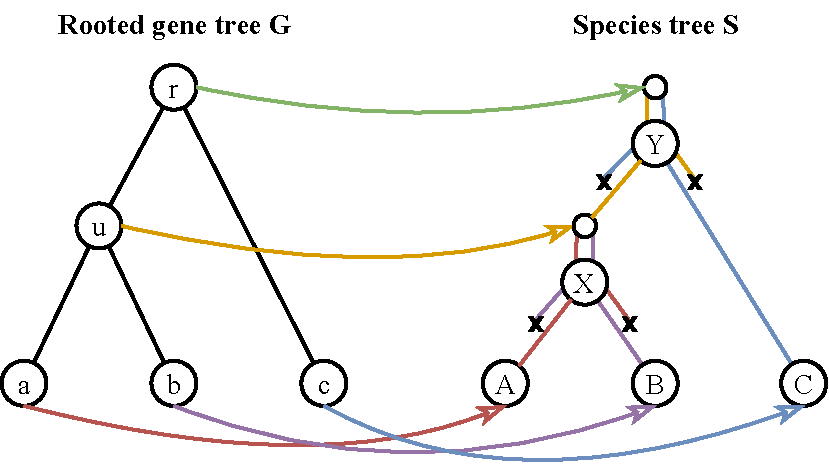
\includegraphics[width=\linewidth]{gene_losses}
  	\caption[Occurrence of gene losses]
  	{On the left is a rooted gene tree $G$ that is mapped to the species tree $S$ on the right. We can see two duplications arising from the mappings $\phi(u)$ and $\phi(r)$, which does not map to its LCA-mapping $\sigma(u)$ and $\sigma(r)$. Each duplication causes two gene losses that occur below species nodes. On the paths from $\phi(a)$ to $\phi(u)$ and $\phi(b)$ to $\phi(u)$, we infer one gene loss on each path due to the species node $X$, where no gene node is mapped. On the paths from $\phi(u)$ to $\phi(r)$ and $\phi(c)$ to $\phi(r)$, we have one gene loss for each path caused by species node $Y$.}
  	\label{gene_losses}
\end{figure}




